\begin{frame}{Finding the Best Line}
    We want a line with small residuals, but if we minimize
    \[
        \sum_{i=1}^n e_i = \sum_{i=1}^n (y_i - \hat{y}_i)
    \]
    we will get very large negative residuals!
\end{frame}

\begin{frame}{Finding the Best Line}
    As with the standard deviation, we will use squares to shift the focus to magnitude:
    \[
        \sum_{i=1}^n e_i^2 = \sum_{i=1}^n (y_i - \hat{y}_i)^2
    \]
    and will find the $\beta$ estimates that minimize this. This is called the \textbf{Least Squares Criterion}.
\end{frame}

\begin{frame}{Finding the Best Line}
    We often call this approach \textbf{least square regression}. To fit this line, we want
    \begin{itemize}
        \item Linearity. The data should show a linear trend.
        \item Nearly normal residuals. The residuals should be well-approximated by a normal distribution.
        \item Constant variability. As we move along $x$, the variability around the regression line should stay constant.
        \item Independent observations. This will apply to random samples.
    \end{itemize}
\end{frame}

\begin{frame}{Finding the Least Squares Line}
    We want to estimate $\beta_0$ and $\beta_1$ in the equation
    \[
        y = \beta_0 + \beta_1 x + \epsilon
    \]
    by minimizing $\sum_{i=1}^n (y_i - \hat{y}_i)^2$.
\end{frame}

\begin{frame}{Finding the Least Squares Line}
    This turns out to be remarkably straightforward! The slope can be estimated as
    \[
        b_1 = \frac{s_y}{s_x}R
    \]
    and the intercept by 
    \[
        b_0 = \bar{y} - b_1 \bar{x}
    \]
\end{frame}

\begin{frame}{Finding the Least Squares Line}
    Although these formulas are easy to write out, they can be cumbersome to work through.
    
    \vspace{12pt}We usually use a computer to find the equation for a least squares linear regression line!
\end{frame}

\begin{frame}{Extrapolation}
    \begin{itemize}
        \item When we make predictions, we simply plug in values of $x$ to estimate values of $y$. 
        \item However, this has limitations!
        \item We don't know how the data outside of our limited window will behave.
    \end{itemize}
\end{frame}

\begin{frame}{Extrapolation}
    Applying a model estimate for values outside of the data's range for $x$ is called \textbf{extrapolation}.
    \begin{itemize}
        \item The linear model is only an approximation.
        \item We don't know anything about the relationship outside of the scope of our data.
        \item Extrapolation assumes that the linear relationship holds in places where it has not been analyzed.
    \end{itemize}
\end{frame}

\begin{frame}{Extrapolation}
    \begin{center}
        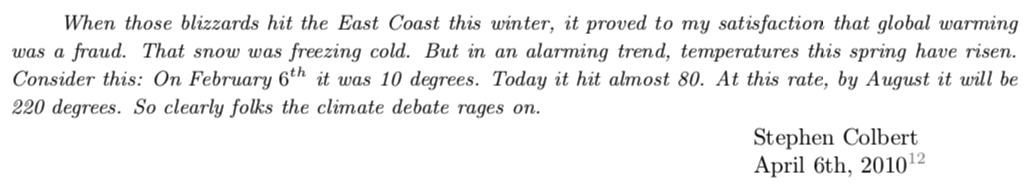
\includegraphics[scale=0.3]{images/colbert.png}
    \end{center}
\end{frame}

\begin{frame}{Using $R^2$ to Describe Strength of Fit}
    We've evaluated the strength of a linear relationship between two variables using the correlation coefficient $R$.
    
    \vspace{12pt}However, it is also common to use $R^2$. This helps describe how closely the data cluster around a linear fit.
\end{frame}

\begin{frame}{Using $R^2$ to Describe Strength of Fit}
    Suppose $R^2 = 0.62$ for a linear model. Then we would say
    \begin{itemize}
        \item About 62\% of the data's variability is accounted for using the linear model. 
    \end{itemize}
    And yes, $R^2$ is the square of the correlation coefficient $R$!
\end{frame}

\begin{frame}{What's good?}
    So what is a good or a bad fit? \\ This will depend a lot on what field you are in!
    
    \vspace{12pt}However, for the purpose of this class, we will use a GPA system:
    \begin{itemize}
        \item $R^2\ge0.9$ is an A fit.
        \item $0.8 \le R^2 < 0.9$ is a B fit.
        \item $0.7 \le R^2 < 0.8$ is a C fit.
        \item $0.6 \le R^2 < 0.7$ is a D fit.
        \item $R^2 < 0.6$ is an F fit.
    \end{itemize}
\end{frame}